\de{Eine natürliche Zahl $n \geq 2$ heisst \emph{resistent}, wenn sie teilerfremd zur Summe ihrer Teiler ist (inklusive $1$ und $n$). Was ist die maximale Anzahl aufeinanderfolgender resistenter Zahlen?}
\fr{On appelle un nombre naturel $n \geq 2$ \emph{résistant} s'il est premier avec la somme de tous ses diviseurs ($1$ et $n$ inclus). Quelle est la longueur maximale d'une suite de nombres résistants consécutifs ?}
\ita{}
\en{A positive integer $n\geq 2$ is called \emph{resistant} if it is coprime to the sum of all its divisors (including $1$ and $n$). What is the maximal number of consecutive resistant numbers?}

\begin{center}
	%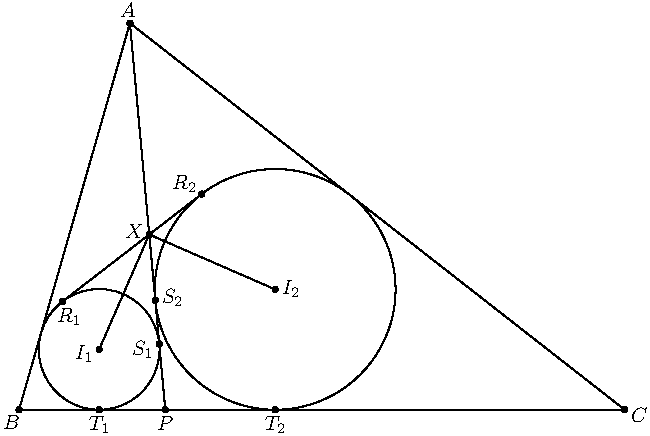
\includegraphics{2022/Final Round/Master Solution/fig-f8.pdf}
\end{center}

\textbf{Solution:} Let $\omega_1$ and $\omega_2$ be the two incircles, centered at $I_1$ and $I_2$ respectively. We first introduce the points $R_1$ and $S_1$ on $\omega_1$ such that $XR_1$ and $XS_1$ are tangent to $\omega_1$, with the condition that $S_1$ is on the line $AP$. Similarly, we introduce the points $R_2$ and $S_2$ on $\omega_2$ such that $XR_2$ and $XS_2$ are tangent to $\omega_2$, with the condition that $S_2$ is on the line $AP$. Finally, let $T_1$ and $T_2$ be the contact points of $\omega_1$ and $\omega_2$ on the line $BC$. Noting that $I_1$,  $I_2$ are on the angle bisectors of $\angle R_1XP$, $\angle PXR_2$, respectively, we find that 
\[
    \angle R_1XR_2=\angle R_1XP+\angle PXR_2=2\cdot(\angle I_1XP+\angle PXI_2)=2\cdot 90^\circ=180^\circ,
\]
so that $R_1R_2$ is a common tangent of $\omega_1$ and $\omega_2$. Note that, by reflection over $I_1I_2$, we have $R_1R_2=T_1T_2$. Moreover, as tangents from a point have the same length, we can observe that
\[
    R_1R_2=R_1X+XR_2=XS_1+XS_2=S_2S_1+2\cdot XS_2
\]
and
\[
    T_1T_2=T_1P+PT_2=PS_1+PS_2=S_2S_1+2\cdot PS_1,
\]
so that $XS_2=PS_1$, and we can calculate
\[
    AX=AS_2-XS_2=AS_2-PS_1.
\]
However, these last lengths can be computed as distances from a vertex of a triangle to a contact point of its incircle. Hence,
\[
    AX=AS_2-PS_1=\frac{AB+AP-BP}{2}-\frac{AP+PC-AC}{2}=\frac{AB+AC-BC}{2},
\]
which is independent from the choice of $P$.

\newpage
\textbf{Marking Scheme:}

The marking is split into two parts. Part A is the identification of $X$ as being on the other common tangent to the incircles and part B is the computation of $AX$. The points of part A are always additive with the points of part B.

\textbf{Part A:} \dotfill ($3$ points)

The following are non-additive.
\begin{enumerate}[label=(a.\arabic*)]
    \item Proving that $\angle I_1PI_2=90^\circ$  \dotfill ($0$ points)
    \item Claiming that $AX=(AB+AC-BC)/2$, the distance to the contact point \dotfill ($1$ point)
    \item Proving that $I_1PI_2X$ lie on a circle \dotfill ($1$ point)
    \item Claiming that $X$ is on another common tangent of $\omega_1$ and $\omega_2$ \dotfill ($2$ points)
    \item Proving that $X$ is on another common tangent of $\omega_1$ and $\omega_2$ \dotfill ($3$ points)
\end{enumerate}

\vspace*{0.6cm}
\textbf{Part B:} \dotfill ($4$ points)

The following are additive.
\begin{enumerate}[label=(b.\arabic*)]
\item Proving that $XS_1=PS_2$, or an equivalent equality \dotfill (1 point)
    \item Computing $PS_1$ in terms of the sides of $ABP$ \dotfill (1 point)
    \item Computing $AS_2$ in terms of the sides of $APC$ \dotfill (1 point)
    \item Conclude \dotfill (1 point)
\end{enumerate}
